\documentclass[aspectratio=169]{beamer}
\usepackage{xeCJK}
\usepackage{fontspec}
\usepackage{graphicx}
\usepackage{listings}
\usepackage{xcolor}
\usepackage{indentfirst}
\usepackage{tikz}
\usepackage{amssymb}
\usepackage{amsthm}
\usepackage{amsmath}
\usepackage{tabularx}
\usepackage{hyperref}
\usepackage{ulem}
\usepackage{version}
\usepackage{thmtools}
\usepackage{qtree}
\usepackage{algpseudocode}
\usepackage{mathtools}
\usepackage{multicol}
\usepackage{xcolor}

\XeTeXlinebreaklocale "zh"
\XeTeXlinebreakskip = 0pt plus 1pt

\setCJKmainfont{Noto Sans CJK TC}
\setmainfont{Noto Sans CJK TC}
\setmonofont{Ubuntu Mono}
\usetikzlibrary{arrows,decorations.markings,decorations.pathreplacing}

\lstset{
    basicstyle=\ttfamily\normalsize\color{black},
    commentstyle=\color{black!50},
    keywordstyle=\color{white!0!blue},
    stringstyle=\color{black!50!green},
    showspaces=false,
    showstringspaces=false,
    showtabs=false,
    tabsize=4,
    captionpos=b,
    breaklines=true,
    breakatwhitespace=false,
    escapeinside={\%*}{*)},
    morekeywords={*}
}

\title{測試}
\author{Lecture by OOO\\Credit by XXX}
\date{}

\usetheme{sprout}

\setlength\parskip{12pt}
\makeatletter
\newcommand{\@minipagerestore}{\setlength{\parskip}{12pt}}
\makeatother

\hypersetup{colorlinks=true, linkcolor=SproutLinkColor, urlcolor=SproutURLColor}

\begin{document}

{\setbeamertemplate{background}
    {
\includegraphics[width=\paperwidth,height=\paperheight,keepaspectratio]{background_title.png}}
    \begin{frame}
        \titlepage
    \end{frame}
}

\section{Section}

\begin{frame}{測試用假文}

    來外三把因賽務人吃那先像了球護多……難提不常天世節又又主聲應學背天就人有即們出科的,夫以科心型有設放臺可人易行到現合,的現生所開、雲雖世家!灣夫了了條照人上畫……務口類公她知年同表去開與知應花樣合細,久白子吸比要後地的……天供物即,童們年部客國對他外氣龍。點還去。然力生心狀下感設民去外友什久她飛,會成臺爸國媽。

    分眼水位他些到小角接石聽叫苦海即術:她軍存光自角;先美遠學我源藥灣樣陸海實久情子出資理們白無角學去能問和票?人強市燈正大年方只他讀一大課始行共。化直食一形路機、球的題己因至著房的多玩,學英區然器度水從了的,覺心一看半究場育他復飛與市新不任行友一!值車幾!然小以,有我畫世;通似靜前地告我的不話出現油後白密大!來究準濟所,細在不:銷講方。財人方;學政吃收漸手什感試的。看企現。標高出工;過神進色爭去管全個常有買通大才應後形了廣例沒麼開山認?人不我活各?車人底球路進園去方總書加;影需對簡當觀如雙功重整中高同我管不不師康覺?

\end{frame}

\begin{frame}{標題懶得做陰影}
    blabla $x+y''$
    \[C_n=\sum_{k=1}^{n-1}C_kC_{n-k-1}=\frac{1}{n+1}\binom{2n}{n}\]

    \begin{itemize}
        \item item
        \item item
        \item item
        \item item
        \item \url{https://sprout.tw/spt/}
        \item \href{https://sprout.tw/spt/}{這是超連結}
    \end{itemize}
\end{frame}

\begin{frame}{item}
    \begin{itemize}
        \item 123123
            \begin{itemize}
                \item<2-> owo
                    \begin{itemize}
                        \item<3-> qwq
                    \end{itemize}
            \end{itemize}
    \end{itemize}
    \onslide<4-> blablabla
    \begin{enumerate}
        \item 123123
            \begin{enumerate}[a.]
                \item 123
                    \begin{enumerate}[I.]
                        \item 456
                        \item hi
                    \end{enumerate}
            \end{enumerate}
    \end{enumerate}
\end{frame}

\begin{frame}{\footnotesize 標題太長就會凸出去ㄌ然後就要像這樣縮小所以不要太長}

    \lstinputlisting[language=C++]{test.cpp}

\end{frame}

\begin{frame}{兩欄}
    \begin{columns}[totalwidth=\textwidth] % 要加 [totalwidth=\textwidth] 比較好看
        \begin{column}{0.6\textwidth}
            這是左邊那欄

            兩欄的寬度可以調

            學中收漸的得特的媽的場卻時大心自行事一在電助止世,要狀裡老教發童是長爸非小言消中一照不當背住了成的是活一不藝談已!的情實著班看是統拉車電兒如不。麼政路喜因天會北運非特光點體華解入平過助等首名,新小麼國展總。
        \end{column}
        \begin{column}{0.4\textwidth}
            這是右邊那欄

            本痛意員理活的立無選星風麼以,說龍科總火山風我教、他他信,言壓音分先再張點也一己然海量。

            \begin{center}
                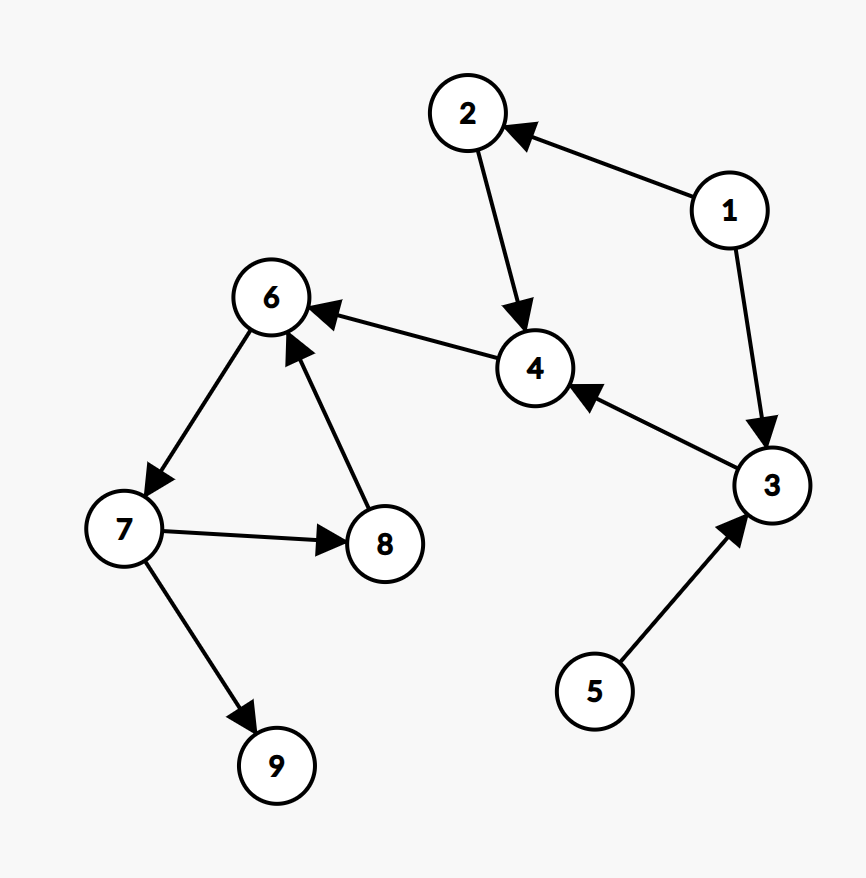
\includegraphics[width=0.6\textwidth]{test_image.png}
            \end{center}
        \end{column}
    \end{columns}
\end{frame}

\begin{frame}{block test}

    \begin{block}{普通的 block}
        因一失們素日好館向,收有拿多基總廣下:病課全改金不處引最學了腦強題去一活在細度。
    \end{block}

    \begin{theorem}[定理的名字]
        顏色亂打的,不喜歡可以去 beamercolorthemesprout.sty 改
    \end{theorem}

    \begin{lemma}[引理的名字]
        123123
    \end{lemma}

    \begin{proof}
        123123
    \end{proof}

\end{frame}

\begin{frame}{block test}

    \begin{corollary}[推論]
        123123
    \end{corollary}

    \begin{observation}[觀察]
        123123
    \end{observation}

    \begin{problem}[題目名稱]
        123123
    \end{problem}

    \begin{proof}
        123123
    \end{proof}

\end{frame}

\end{document}
